% within the first two pages, show a picture / have motivating example
%
% everything is shown at once. not a subset like facet_*()!!
%
% go through features
%   not code related
%
% examples
%   build up data
%   describe plot
%   describe plot results



\documentclass[article]{jss}

%%%%%%%%%%%%%%%%%%%%%%%%%%%%%%
%% declarations for jss.cls %%%%%%%%%%%%%%%%%%%%%%%%%%%%%%%%%%%%%%%%%%
%%%%%%%%%%%%%%%%%%%%%%%%%%%%%%

%% almost as usual
\author{Barret Schloerke\\Purdue University \And
        Second Author\\Plus Affiliation}
% \title{A Capitalized Title: Something about a Package \pkg{foo}}
\title{A Capitalized Title: Something about a Package \pkg{GGally}}

%% for pretty printing and a nice hypersummary also set:
\Plainauthor{Barret Schloerke, Second Author} %% comma-separated
% \Plaintitle{A Capitalized Title: Something about a Package foo} %% without formatting
\Plaintitle{A Capitalized Title: Something about a Package GGally} %% without formatting
% \Shorttitle{\pkg{foo}: A Capitalized Title} %% a short title (if necessary)
\Shorttitle{\pkg{GGally}: A Capitalized Title} %% a short title (if necessary)

%% an abstract and keywords
\Abstract{
  The abstract of the article.
}
\Keywords{keywords, comma-separated, not capitalized, \proglang{Java}}
\Plainkeywords{keywords, comma-separated, not capitalized, Java} %% without formatting
%% at least one keyword must be supplied

%% publication information
%% NOTE: Typically, this can be left commented and will be filled out by the technical editor
%% \Volume{50}
%% \Issue{9}
%% \Month{June}
%% \Year{2012}
%% \Submitdate{2012-06-04}
%% \Acceptdate{2012-06-04}

%% The address of (at least) one author should be given
%% in the following format:
\Address{
  Barret Schloerke\\
  Department of Statistics\\
  Purdue University\\
  250 N. University St.\\
  West Lafayette, IN
  47906
  USA\\
  E-mail: \email{schloerke@gmail.com}\\
  URL: \url{http://ggobi.github.io/ggally}
}
%% It is also possible to add a telephone and fax number
%% before the e-mail in the following format:
%% Telephone: +43/512/507-7103
%% Fax: +43/512/507-2851

%% for those who use Sweave please include the following line (with % symbols):
%% need no \usepackage{Sweave.sty}

%% end of declarations %%%%%%%%%%%%%%%%%%%%%%%%%%%%%%%%%%%%%%%%%%%%%%%

\begin{document}

%%%%%%%%%%%%%%%%%%%%%%%%%%%%%%%
%% include your article here, just as usual
%% Note that you should use the \pkg{}, \proglang{} and \code{} commands.
%%%%%%%%%%%%%%%%%%%%%%%%%%%%%%%

% \section[About Java]{About \proglang{Java}}
%% Note: If there is markup in \(sub)section, then it has to be escape as above.

% # Paper
% * (< 25 pages including everything)
%   * can include things in supplementary location
%     * is free to the internet
%   * must flow together
%     * not many side stories of technical details
%     * can put these in appendix section


% \section[Literature Review]{Literature Review}
\section{Introduction}
  % * (1 - 2 pages; setup work; get excited; )
  % * GGally / ggpairs
  %   * emerson paper
  %   * linked scatter plots / cleveland

  ``The R package \pkg{ggplot2} is a plotting system based on the grammar of graphics. \pkg{GGally} extends \pkg{ggplot2} by adding several functions to reduce the complexity of combining geoms with transformed data.
  Some of these functions include a pairwise plot matrix, a scatterplot plot matrix, a parallel coordinates plot, a survival plot, and several functions to plot networks.''

The focus of this paper explores the function \code{ggduo}, which makes a two grouped plot matrix.

  ``generalized pairs plot
    expanded the traditional scatter plot matrix to work for both continuous and categorical columns.''

  \code{ggduo}'s older brother, \code{ggpairs}, has already been been used in
    \cite{cook2016data}
    \code{ggs_pairs} from \cite{xavier2016ggmcmc}
    and a reverse dependency in over twenty other packages on CRAN and BioConductor.




\section[Methodology]{Methodology}
  % * (5-10 pages)
  % * (conceptual framework)
  % * (guts of the program)
  % * How ggmatrix is a general structure to accommodate ggpairs and now ggduo


    A scatterplot matrix shows the same collection of data in each panel of a plot matrix, however each panel has different continuous axes.
    Similarly, the generalized pairs plot displays the same collection of data using different axes but allows for a mix of plotting methods and both continuous and discrete plot axes.
    \code{ggduo} removes the restriction plotting all pairs of points and displays the combination of two groups of the same dataset.

    With \code{ggduo}, a scatterplot can be next to a boxplot, which can be next to a mosaic plot.

\subsection{What is ggduo}

\code{ggduo} is function in the GGally package that produces a ggmatrix plot matrix with one column of data plotted against another column of data for every panel of a plot matrix.
For a given row, the same y axis variable is used, and for a given column, the same x axis variable is used.
Unlike ggpairs, the restriction of every column being paired against every column is removed.
\code{ggduo} only requires a set of `Y` columns and a set of `X' columns to be paired against each other.



\subsection*{Column types}

\code{ggduo} inspects and displays the data columns according to their variable type: continuous or discrete.
There are three plot type groups that an be made from these two options: continuous vs. continuous, continuous vs. discrete, and discrete vs. discrete.
\code{ggduo}'s default plotting behavior for continuous vs. continuous is to produce a scatterplot with a loess smooth curve displayed on top of the points.
The default plotting behavior for discrete vs. discrete, is to summarize the data and display it as a mosaic plot.

The third group, continuous vs. discrete, will be refered to as a `combination plot'.
\code{ggduo} makes a distinction between the two possible combination plots: continuous vs. discrete (vertical combination plot) and discrete vs. continuous (horizontal combination plot).
By default, \code{ggduo} displays grouped histograms for a horizontal combination plot and grouped box plots for a vertical combination plot.
This distiction between a horizontal and vertical combination plot is made as there are no plot matrix sections (upper, lower, diagonal) in a \code{ggduo} plot.




\subsection{User defined functions}

The default plotting functions are provided by the GGally package, however the user may use their own plotting functions for each panel.
Example!!


Each of these panels are full ggplot2 and are stored in a ggmatrix object which will be talked about in the next section.


\subsection{Plot matrix}

  Winston Chang explains facet'ing as ``[ploting] subsets of data into separate panels'' \cite{chang2013rgc}.
  With ggplot2's faceting, each piece of data is displayed only once per plot matrix with the same plotting method and same axes.
  On the other hand, GGally's \code{ggduo} displays the same piece of data in every panel but with different axes and different plotting methods.
  As stated earlier, each column of the plot matrix shares the same x axis variable and each row of the plot matrix shares the same y axis variable


  ggplot2 prevents discrete scales from being mixed with continuous scales.
  This idea makes sense when looking at a single panel plot or a multiple panel plot with different subsets of the same data.
  The ability to display different axes natively in the same plot matrix is not possible with ggplot2.
  However, only one scale type is used per ggmatrix panel, so the original `per panel' logic is still kept.
  Before a ggmatrix object, to have two, related mixed axes plots in the same display could only be done with \pkg{gridExtra} or \pkg{grid}.
  Neither of these packages would produce output with the native ggplot2 presence.


  \code{ggmatrix} extends the \code{facet_grid} idea but allows for a different scale per row and column.
  This allows for a cohesive plot matrix structure where all axes are shared among common parts.


  Mixing different plot types allows the user the digest their data with multiple ways with the same display.


  To be able to mix axes arbitrarily, the GGally package uses a ggmatrix object.
  It contains a collection of plot objects and other plotting features such as number of columns and rows, title, labels, etc.
  Each plot is displayed in a cell of a plot matrix with the same contruction as a ggplot2's \code{facet_grid()} plot matrix.
  There are strips on the top and right side of the plot matrix, and plot axes are only displayed on left and bottom side of the plot matrix.
  Like with ggplot2, space can be made available for the legend, title, x label, and y label.




  %  that can be displayed to
  % Like with ggpairs,


  % ggplot2 displays data with the same axis size even if the type of plot changes.  Leveraging this fact, each plot is displayed with independent axis knowledge.

  % limitation of ggplot2. all continuous scale or all same category. no mixing
  %   able to create the same plot for different subsets of data with ggplot2
  %   unable to combine two related plots in the same display without use of \pkg{gridExtra} or \pkg{grid}
  %
  % plots may be retrieved individually. not possible with ggplot2
  %
  % core of plot matrix is a ggmatrix object
  %   generalized plot matrix.
  % plots are arbitrary
  %   composite plot \cite{emerson2013gpp}
  %   allows for plots with completely different scales to be shared in the same matrix
  %
  % output is modeled directly after \pkg{ggplot2}'s \code{facet_grid}
  %   columns
  %   rows
  %   strips (titles)
  %   general plot behavior
  %   allows for legends and uses the ggplot2 formatting
  % similar to ggplot2, meta information is stored in the plot matrix until print time and may be altered after it's inception.
  %
  %
  % similar to ggpairs, \code{ggduo} formats the plot objects to be displayed with ggmatrix
  % inherits all the functionality of ggmatrix


\newpage

\section[Examples]{Examples}
  % * (<= 5 pages)
  % * (breadth of application)



\subsection{Canonical correlation analysis}
% * CCA

  Canonical correlation analysis is a method to analyize the correlation between two matrices \cite{hotelling36cca}.
  Canonical correlation analysis can be directly displayed with \code{ggduo}.
  Before \code{ggduo}, canonical correlation analysis did not have a cohesive plotting mechanism to visually display the associations of two sets of mixed type variables.
  Current examples use `ggpairs' to display all pairs of columns when only a subset of combinations are needed.
  `ggpairs' can be used to check the within correlation of both the explanatory variables and response variables,  whereas \code{ggduo} can be used to check the correlation between the explanatory and response variables.
  Using ggmatrix's power of independent plots, each cell can display custom plots to show any information.


  Explain academic data here

  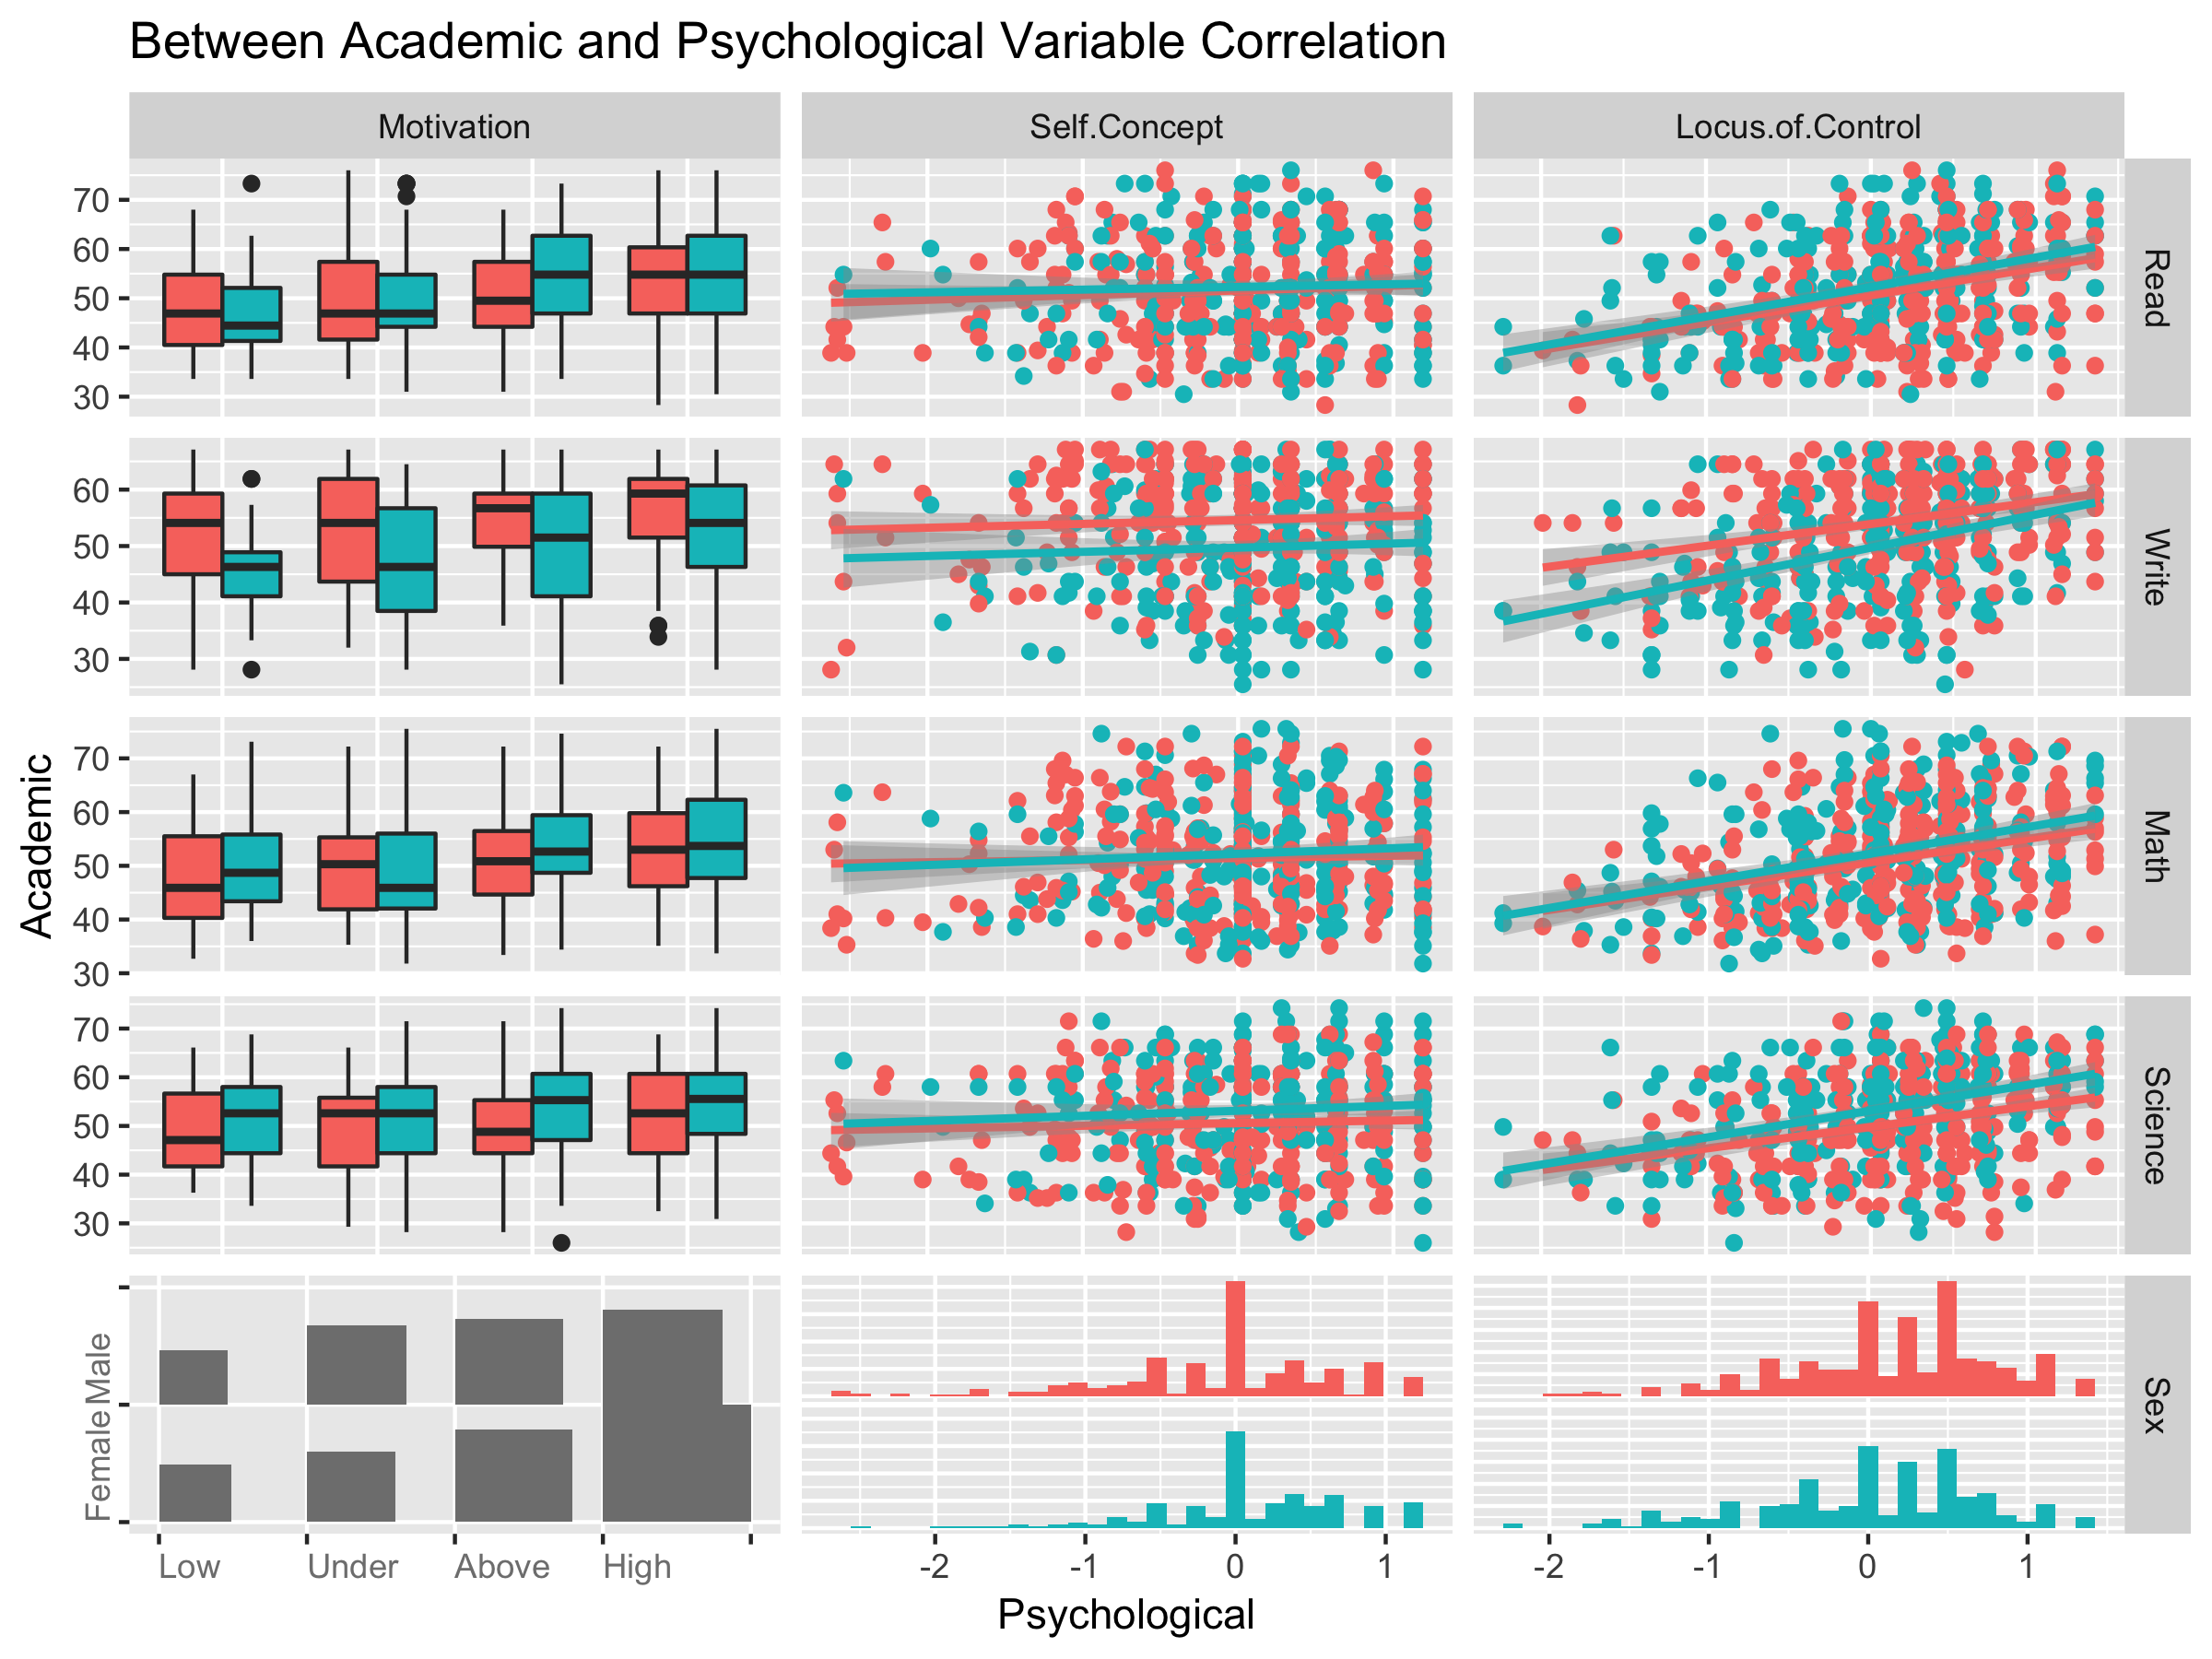
\includegraphics{imgs/cca.png}



  \subsection{Multiple Time Series Analysis}
  % * Time Series
  %   * break temporal components

  The \pkg{stats} package has a \code{ts.plot} function that currently allows for multiple time series to be printed in a single plot.
  Display the time axis on the X axis with multiple columns on the Y axis.
  \code{ts.plot} displays the data in the same plot panel with a shared Y axis.
  Displaying the data on the same axis does not make sense in all cases.
  Splitting the multiple time series plot along the Y axis, we can display multiple panels with different Y axes with a shared X axis using \code{ggduo}.
  This can be done with \code{ggts} which wraps to \code{ggduo} with the X column label turned off by default and a plot X label of `time'.

  Explain pigs data here

  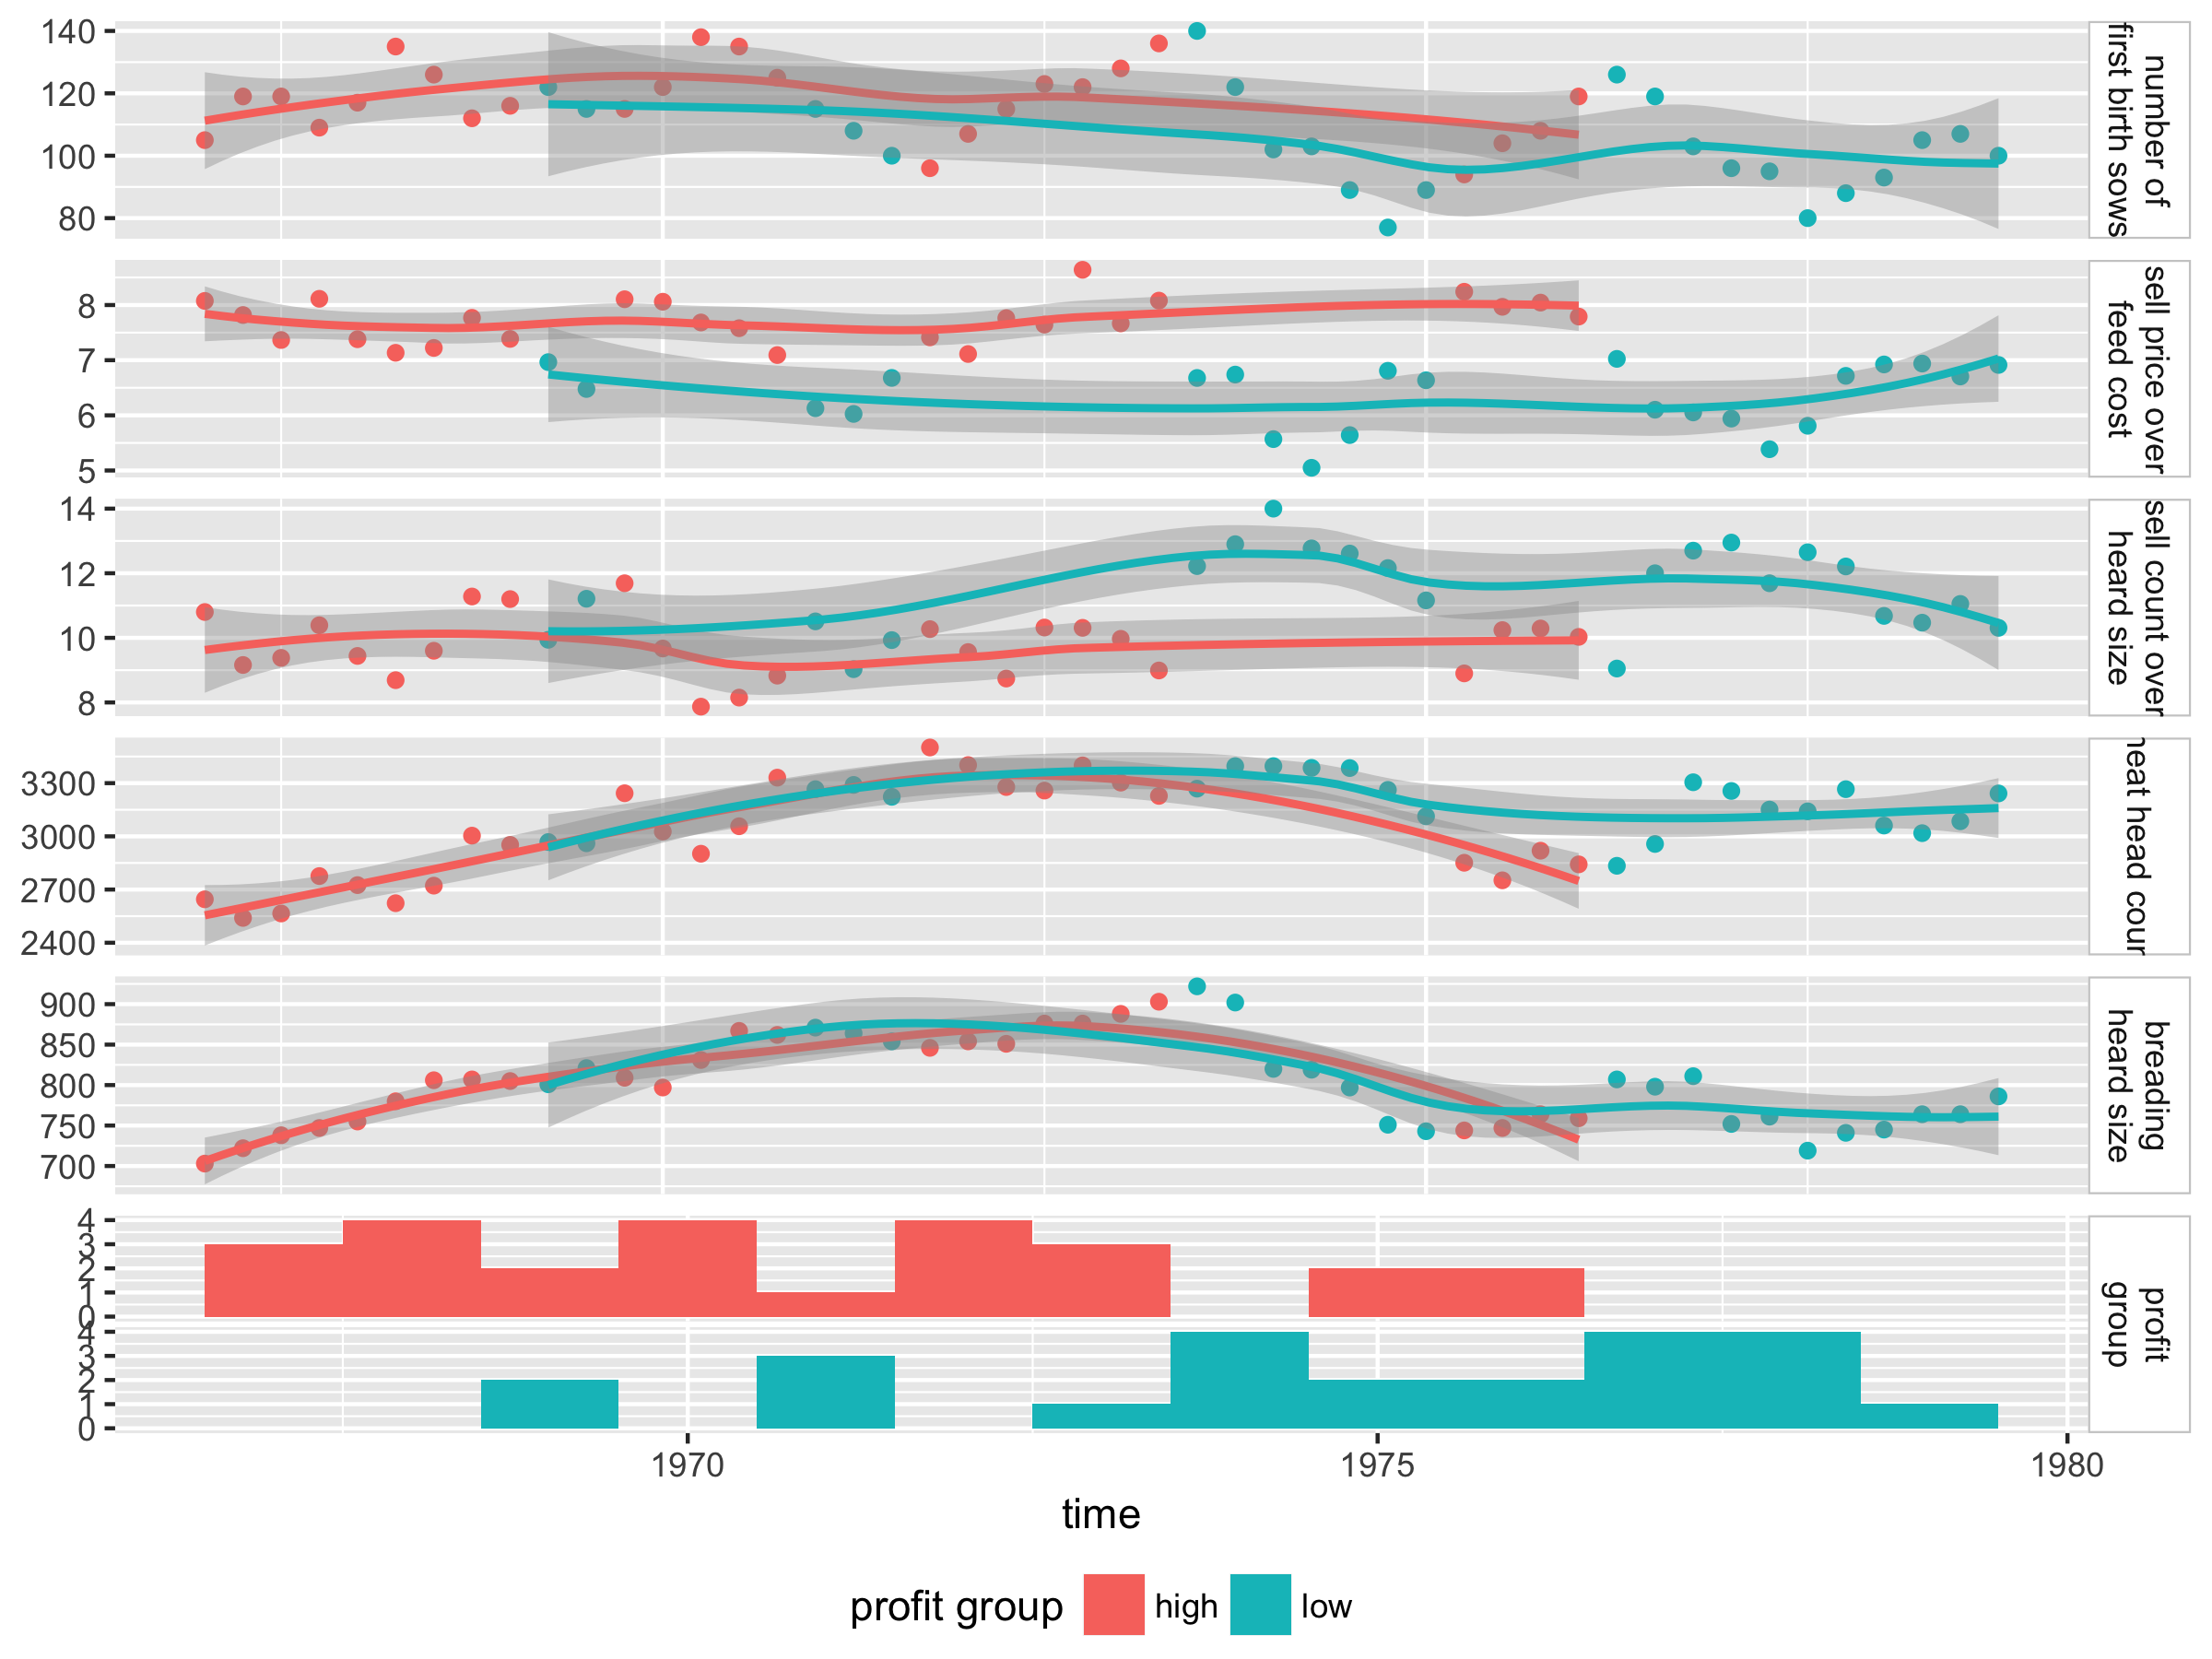
\includegraphics{imgs/pigs.png}




\subsection{Multiple regression diagnostics}

% * Regression
%   * marginal model
%   * residuals
%   * cooks distance
%   * (other 'y' sections)

Multiple regression analysis is currently being done using ggpairs and only needs to display a subset of the pairs of columns.
With the basis of ggduo displaying each row of the data in every panel with different functions, ggduo quickly extends to model diagnostics.
There are many diagnostics that can be calculated for each row of explanatory data.
By default, \code{ggnostic} (a function that wraps around \code{ggduo}) looks at the residuals, leave one out sigma value, leverage points, and Cook's Distance.
Each diagnostic information is plotted against all explanatory variables used in the model.

Using stats::step to determine a best fitting model, the default diagnostics are displayed against `species', `tars1', `tars2', and `aede'.
The residuals have a 95\% confidence interval in dashed lines and a solid line at 0.
The leave one out sigma value displays a solid line for the current model's sigma value.
The leverage points (hat) are centered around the solid line at $p / n$ and have a dashed line at $2 * p / n$.
Finally, the Cooks's distance has a grey dashed line at $4 / n$.
Each solid line corresponds to the expected value and each dashed line corresponds to a `signifigance' cuttoff value.
The asterisks in the X axis strips corresponding to the significance of an anova F test.

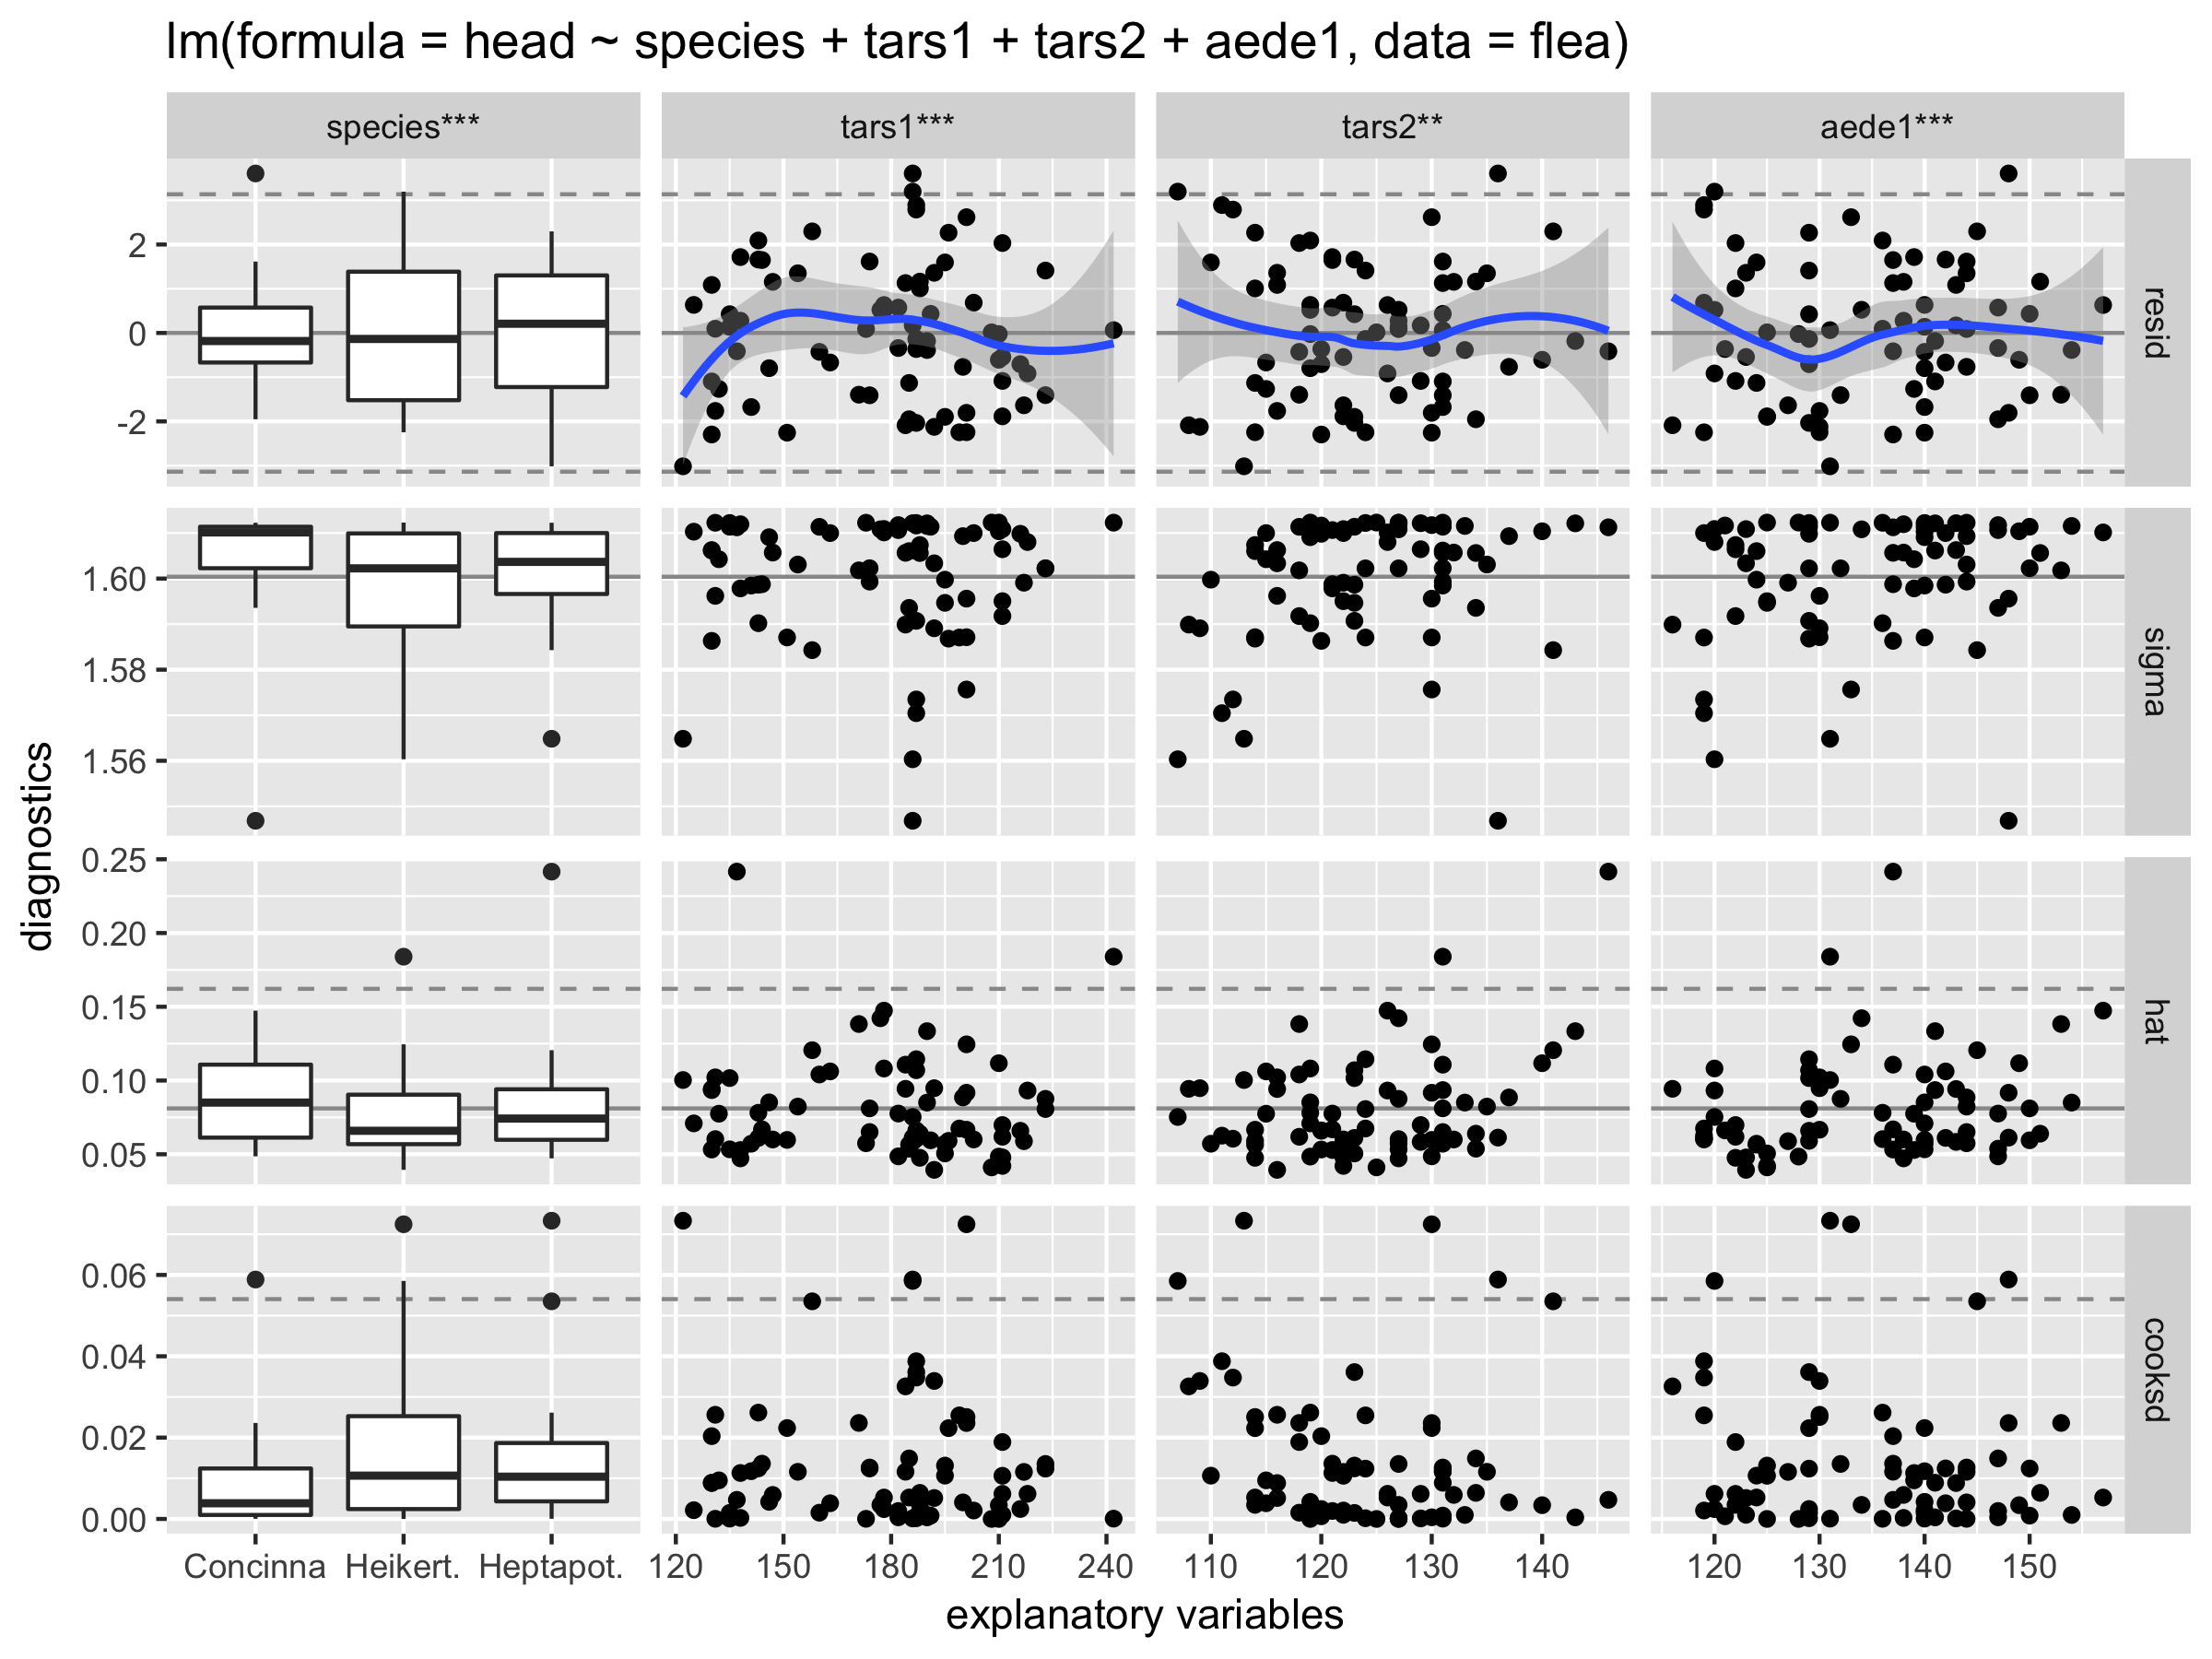
\includegraphics{imgs/ggnostic_plain.png}

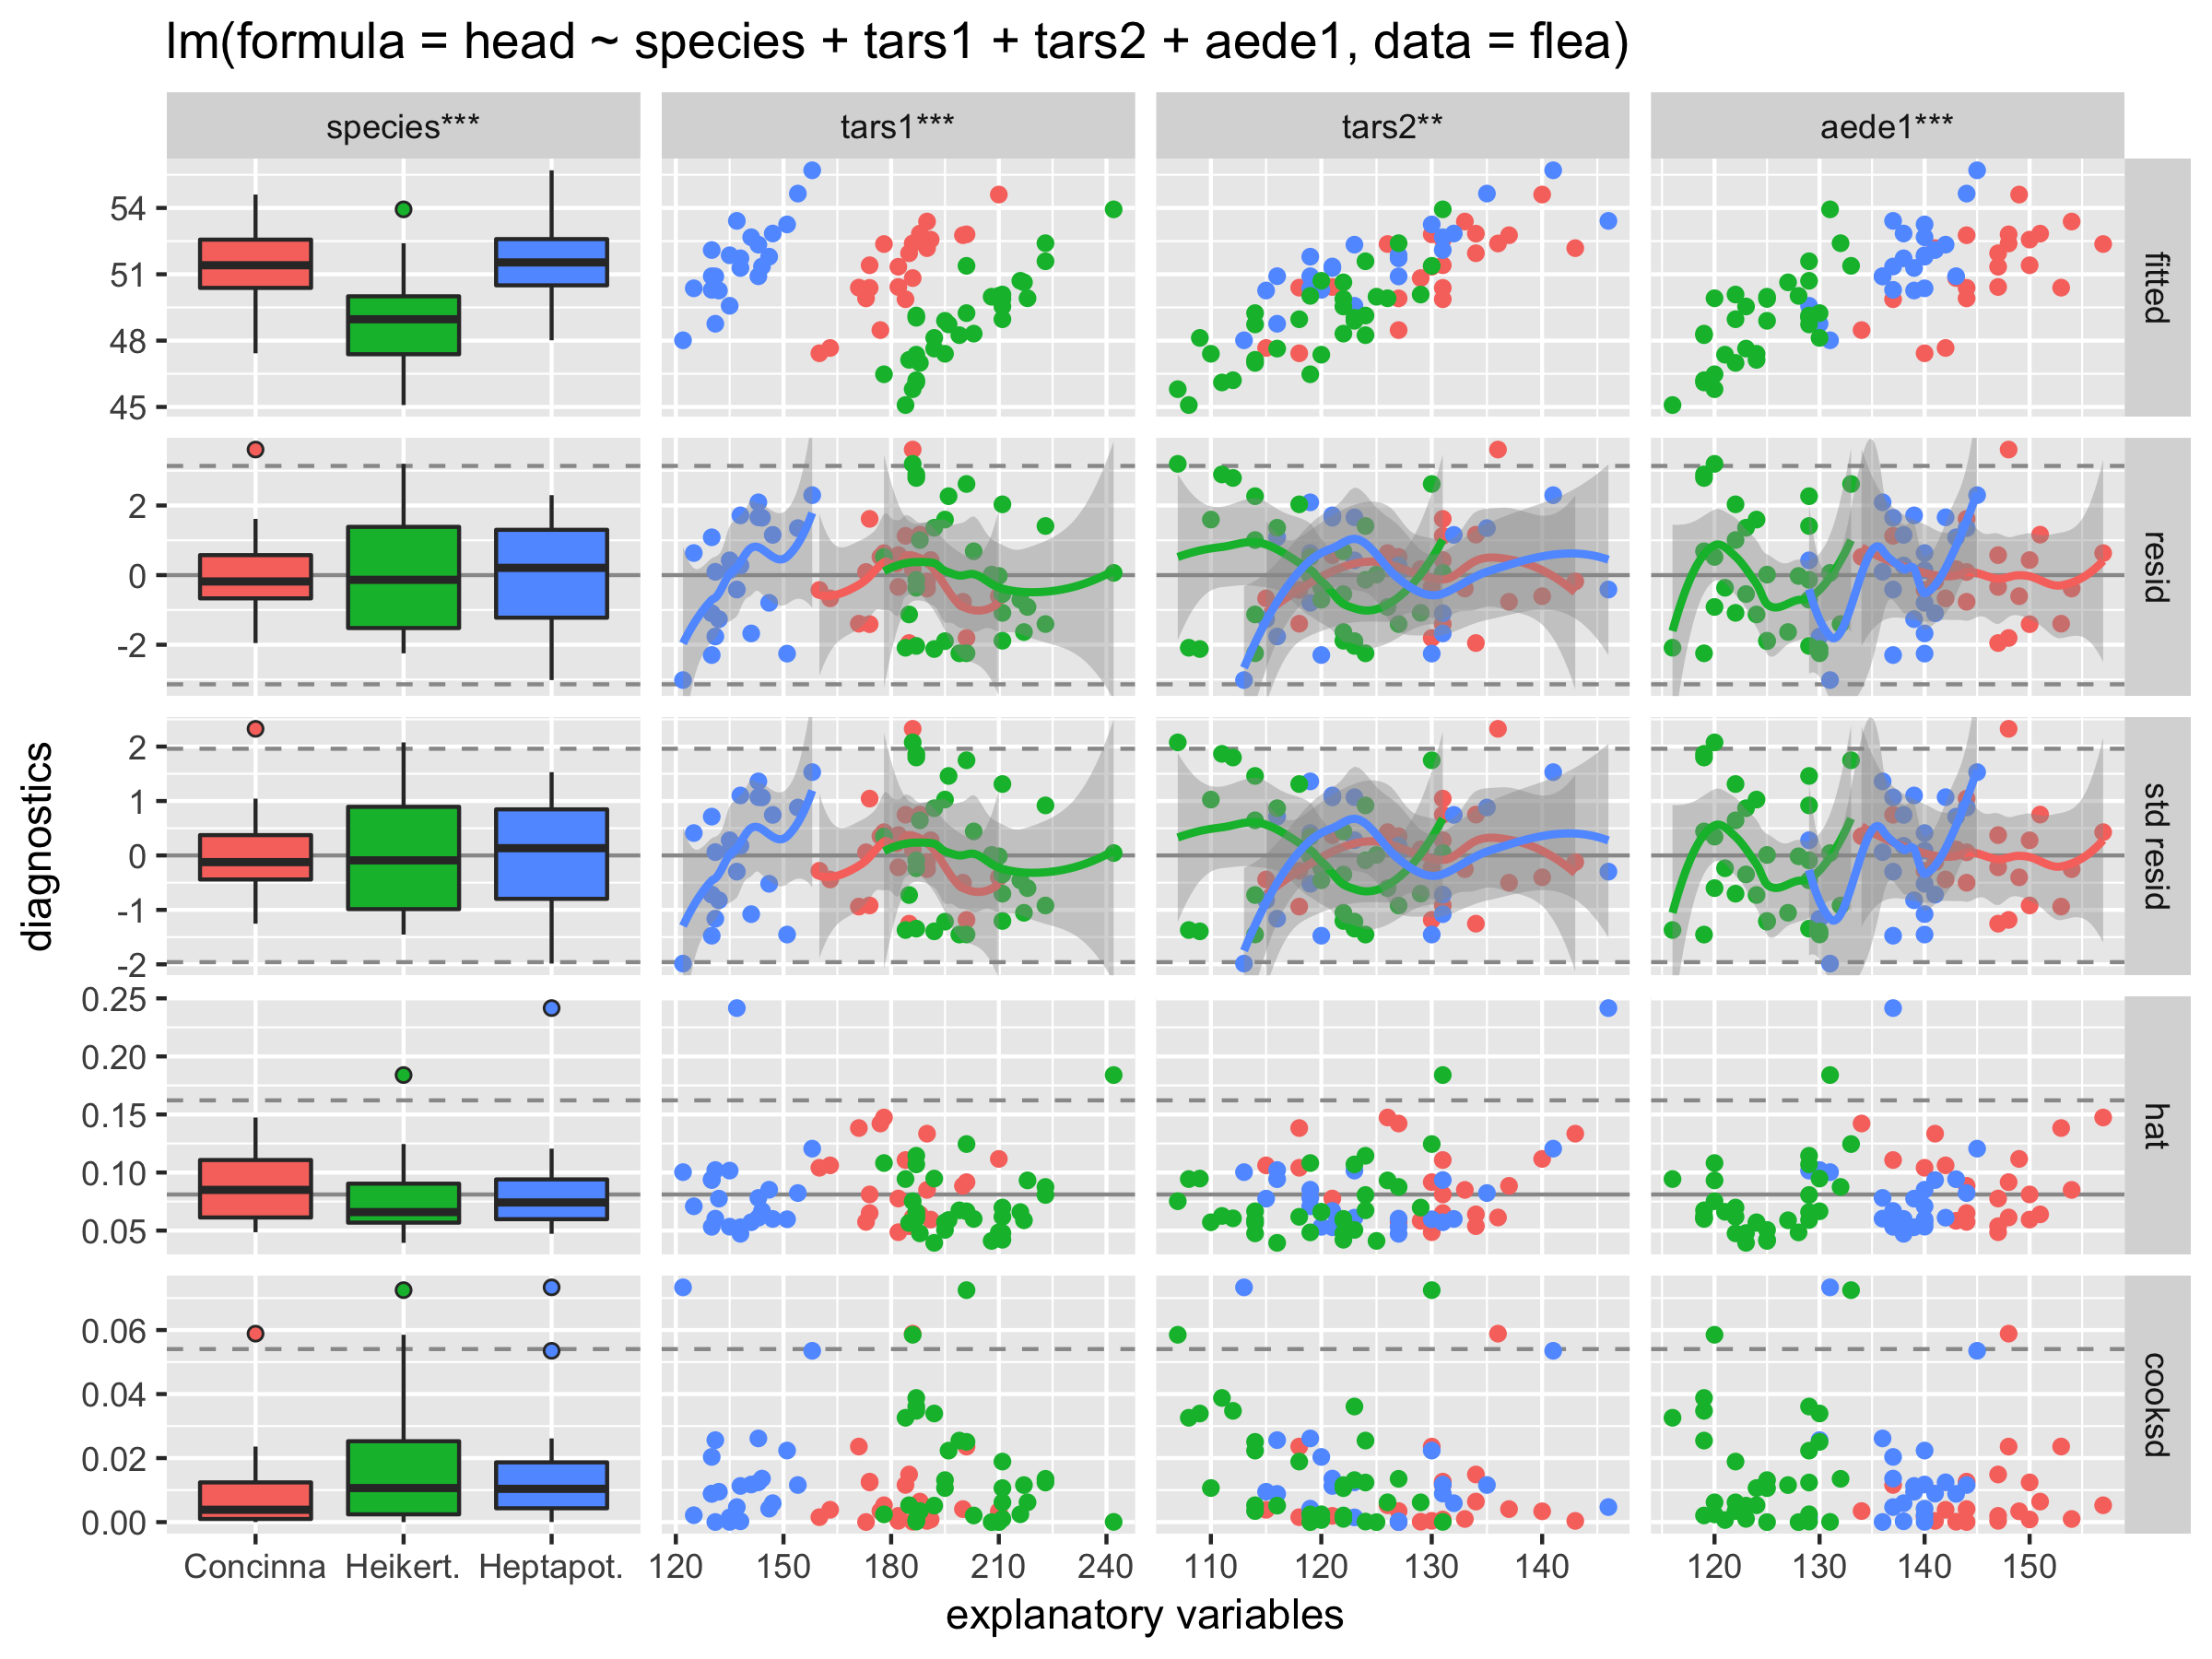
\includegraphics{imgs/ggnostic_complex.png}


  % * Interaction
  %   * plot.ly
  %   * Ties back to cleveland's linked scatterplots






\section[Future Direction]{Future Direction}
% * (<= 1 pages)
Currently all individual plots are rendered at run time.  \pkg{ggplot2} is known for having slower print speeds.
currently printing n*m plots takes time.

Future ggplot2 versions will allow for custom faceting.  this could potentially allow ggmatrix to print a single ggplot2 object with custom facet scales for each plot.  This would dramatically reduce the amount of time a ggmatrix takes to render.  Printing time would still remain the same.

Link up with the javascript packages for interactive plot matricies. Would be great to add a one more line of code to turn it into an interactive plot.


\section[Discussion]{Discussion}
% * (<= 1 pages)
%   * pros and cons
Pros
  single line of code to produce a composite plot matrix
  works well with wide data
Cons
  takes longer time to print with larger data
  prints m*n ggplots to produce a single m*n plot matrix

%   * origin and why it came about
  ggmatrix
    was a feature request to handle different length and different column plot matrix
    users wanted to place custom plots in a custom arrangement
  ggduo came about
    was a feature request to have a ggmatrix version of the TeachingDemos::pairs2 function.

%   * what we can not achieve with the ggmatrix / ggduo
Can achieve custom plots.
Can not achieve a forced cohesive scale to be used on all plots in a row or column
is not a native ggplot2 object, but trying hard to be like one!

\section[References]{References}
  % * (1 - 2 pages)

  \bibliography{article}

\end{document}
